\subsection{Aufbau der UHV-Apparatur}

Der Sprühbeschichter soll auf der bisher vorhandenen Ultrahochvakuums-Apparatur (siehe Abb
\ref{uhvaufbau}) aufgebaut werden.~%, in der das Substrat präpariert werden kann.
 Diese besteht aus mehrerern Kammern, die untereinander verbunden sind. Die gesamte Apparatur ist
auf vier Druckluftfüßen gelagert, um über den Boden übetragende störende Schwingungen zu minimieren. Um ein
Ultrahochvakuum im Bereich von $10^{-10}$mbar zu erzeugen, kann die Apparatur zunächst mit einem
mobilen Pumpstand %(hier verwendet: HiCube von Pfeiffer ) 
auf ein Hochvakuum im Bereich von
$10^{-7}$mbar gepumpt werden; ab einem Druck von $10^-6$mbar lässt sich eine fest installierte
Ionengetterpumpe hinzuschalten.

\begin{figure}[H]
\centering
\includegraphics[width=5cm]{uhv.png}
\caption{\textit{Afubau der UHV-Apparatur. }}
\label{uhvaufbau}
\end{figure}

Die Apparatur besteht im wesentlichen aus drei wichtigen Kammern (siehe Abb. \ref{img:uhvkammern}): 
der 
Molekülkammer (1), der STM-Kammer (2) und der Hauptkammer (3). In der Molekülkammer kann die eingebrachte
Probe mit Hilfe des Molekülverdampfers (der in dieser Arbeit nicht verwendet wurde) bedampft werden.
Zukünftig soll auf diesen Teil der Kammer der im Rahmen dieser Bachelorarbeit gebaute
Sprühbeschichter aufgesetzt werden. Dieser Teil der Kammer kann über zwei Ventile von den anderen
Kammern abgetrennt werden.\\
In der STM-Kammer kann die Probe
mittels Rastertunnelmikroskopie- und spektroskopie untersucht werden. In der Haupkammer kann die
Probe durch einen unten in der Kammer eingebauten Metallverdampfer mit
verschiedenen Metallen (Gold, Eisen, Kobalt) bedampft, durch Erhitzen von Ablagerungen auf der
Oberfläche gereinigt ("`geflasht"') sowie die Probenoberfläche durch LEED untersucht werden. Die
hier verwendete LEED-Apparatur ist ein "`Spectaleed"'  von Omicron. 
%Weiterhin sind hier Augerspektroskopie und Kerr-Messung möglich, die jedoch hier nicht zum Einsatz
%kamen.
\\
Das verwendete Substrat kann im Probenhalter mittels des
Transferstabs durch die Kammern transportiert werden. In die Molekülkammer kann er mit einem
weiteren, kleineren Transferstab gesetzt werden. Ein Transfer zum Probentisch des STMs in der
STM-Kammer ist mit Hilfe des sogenannten Wobblesticks möglich, mit dessen Greifzange die Probe an der Probennase gehalten und in
den STM-Tisch versetzt werden kann. In der Hauptkammer schlussendlich wird der Probenhalter in den
sogenannten Manipulator gesetzt, mit dem die Probe in alle Raumrichtungen verschoben sowie gedreht
werden kann. \\
Am Manipulator ist ein Heizfilament angebracht, über den der Kristall geflasht wird:
Dabei wird das Filament zum Glühen gebracht, die durch Glühemission emittierten Elektronen werden
durch eine an die Probe angelegte Hochspannung zum Kristall hin beschleunigt und heizen diesen dann
durch Stöße bis zum Glühen auf. In diesem Prozess werden aufgedampfte Schichten, aber auch
Ablagerungen entfernt. Selbst bei einem Druck von $10^{-10}$mbar lagern sich Restgasmoluküle auf
Oberflächen ab; nach einem Tag entspricht dies in etwa einer Monolage.\\
Weiterhin kann das Filament dazu benutzt werden, ohne angelegte Hochspannung die Probe einfach nur
zu erwärmen ("`tempern"'). Dies kann die Oberflächenstrukturen nach Aufdampfen eines Metalls
deutlich ändern. Die erreichte Temperatur lässt sich aus dem Filamentstrom bestimmen.\\
 Über dem Metallverdampfer in der Hauptkammer befindet sich eine
Schutzklappe, sodass die darüber befindliche Probe durch Auf- oder Zuklappen je nach Bedarf bei
laufendem Verdampfer bedampft werden kann. Die Menge des verdampften Metalls wird über einen
Schwingquarz gemessen, der sich über dem Verdampfer befindet und somit mitbedampft wird; anhand der
Änderung der Schwingfrequenz können Rückschlüsse auf die abgelagerte Masse auf dem Quarz gezogen
werden, worüber dann die Anzahl der aufgedampften Lagen auf der Probe bestimmt werden kann
\cite{Sau}.
Nach Skalierung wird hierfür die digital angezeigte Periodendauer genutzt, dabei entsprechen für Gold
z.B. 250 Skaltenteile etwa einer Monolage Gold auf der Probe.\\
Der Druck in der Hauptkammer wird über eine Bayard-Alpart-Röhre gemessen, die sich unten in der
Kammer befindet. Zudem befindet sich ein weiteres Druckmessgerät %\ldots 
an der Molekülkammer.
Zur Restgasanalyse und Lecksuche dient ein Massenspektrometer.% (Pfeiffer Vacuum PrismaPlus QMG220).


\subsection{Das Rastertunnelmikroskop}

Das hier verwendete Rastertunnelmikroskop ist ein Micro-STM der Firma Omicron. Es besteht
prinzipiell aus einem Röhrenscanner mit einer STM-Spitze aus Platin-Iridium-Draht und einem
Probentisch, über den der Probenhalter bewegt werden kann (siehe Abb. \ref{stmaufbau}). Sowohl der
Röhren\-scanner als auch der Probentisch werden über Piezoelemente bewegt, mit denen sowohl Scanner
als auch Tisch in x-y-Richtung bewegt werden können, der Scanner zum Rastern der Oberfläche und der
Tisch zum Ausrichten der zu messenden Stelle der Probe; weiterhin kann der Scanner in z-Richtung an
die Probe angenähert werden.

% der Scanner in z-Richtung an die Probe angenähert sowie
% zum Rastern der Oberfläche in x-y-Richtung bewegt und der Probentisch in x-y-Richtung
% ausgerichtet werden kann.
Die Steuerung erfolgt über eine Fernbedienung.
Die Spitze des STMs wird dabei so nah wie möglich an die Probe herangefahren, was über die
Spiegelung der Spitze in der Probe, gefilmt über eine schräg unterhalb des Probentisches angebrachte
USB-Kamera, abgeschätzt werden kann. Die Feinanpassung wird über die zugehörige Software erledigt.
Dabei wird die Spitze in kleinen Schritten soweit angenähert, bis ein Tunnelstrom gemessen werden
kann. Anschließen wird die Probe wiederum manuell noch zwei bis drei Schritte weiter an die Probe
herangefahren, um den Tunnelstrom zu stabilisieren.\\

\begin{figure}[H]
\centering
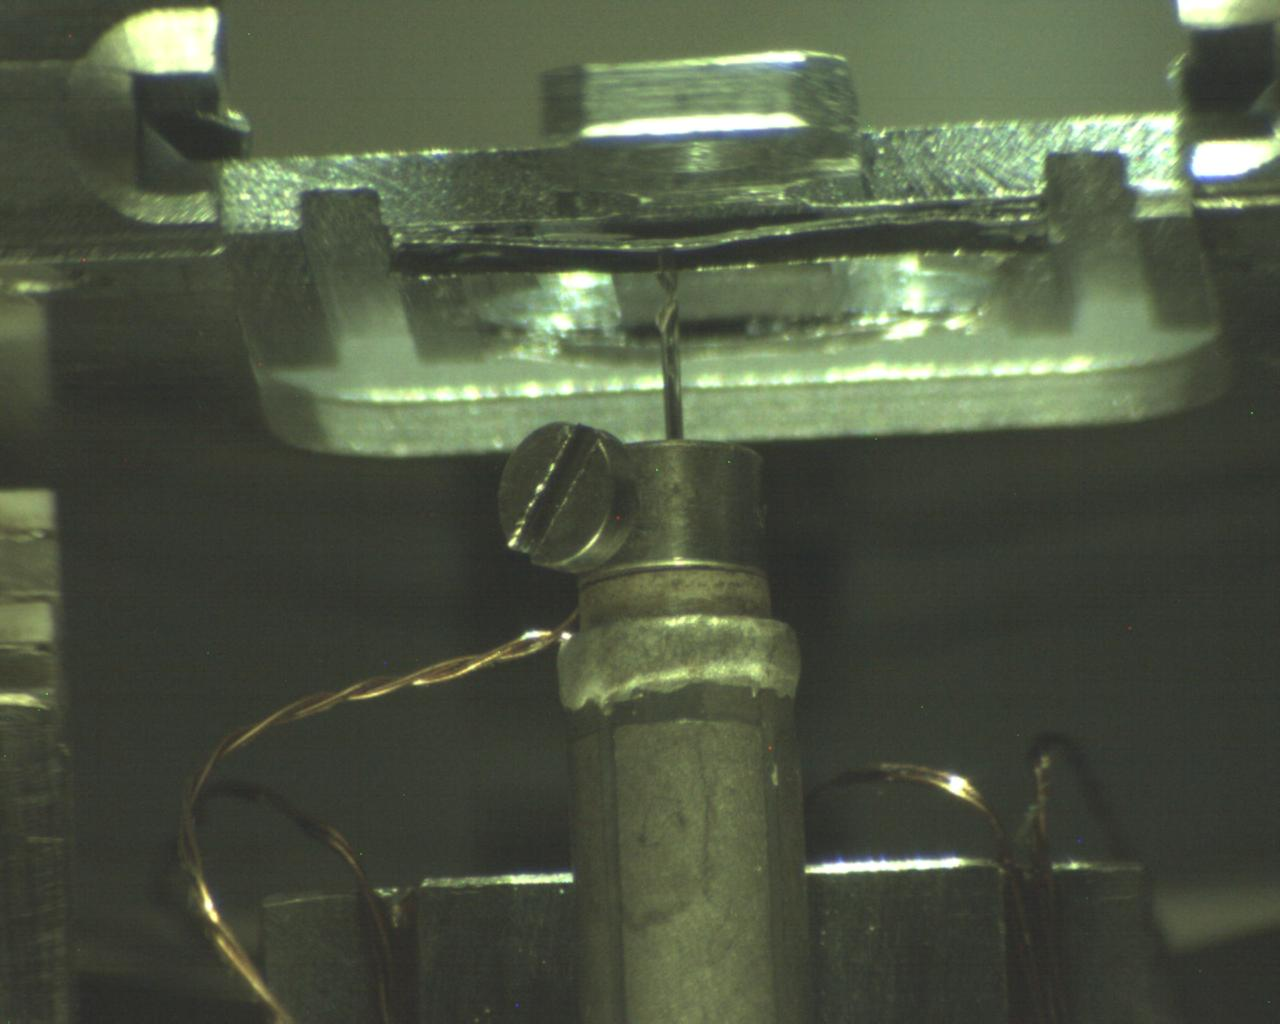
\includegraphics[width=5cm]{kamera2.jpg}
\caption{\textit{bla
}}
\label{stmaufbau}
\end{figure}

Grundsätzlich gibt es zwei Messmethoden. Im Konstathöhenmodus wird der Abstand zwischen Spitze und
Probenoberfläche konstant gehalten. Die Messgröße ist der Tunnelstrom, der im resultierenden
Scanbild als Helligkeitskontrast dargestellt wird. Diese Einstellung ermöglicht eine relative hohe
Scangschwindigkeit, da die Höhe der Spitze nicht nachreguliert werden muss, eignet sich
allerdings auch nur für sehr ebenmäßige Oberflächen, da die Gefahr einer Kollision bei Erhöhungen
der Oberfläche oder die eines Verlusts des Tunnelkontakts bei Mulden besteht.\\
Beim Konstantstrommodus wird der Tunnelstrom durch ständiges Nachregulieren der Höhe konstant
gehalten. So erhält man ein Höhenprofil für die abgerasterte x-y-Ebene, welches ebenfalls durch
Helligkeitskontraste dargestellt wird. Hierbei können auch unregelmäßige Oberflächen gescannt
werden. Zu bemerken ist, dass das scheinbar topographische Bild eigentlich die elektronische
Zustandsdichte der Oberfläche widerspiegelt.




\subsection{Aufbau des Sprühbeschichters}
\FloatBarrier

Der Sprühbeschichter funktioniert im wesentlichen über ein Druckgefälle innerhalb seines Aufbaus, durch das
die in einer Lösung gelösten Moleküle auf das Substrat "`gesaugt"' werden und sie dort im besten
Falle haften bleiben. 
\begin{figure}
\centering
\includesvg{wuerfel}
\caption{\textit{Der Aufbau des Sprühbeschichters. 
%Zwischen Würfel und unterem Teil der Kammer,
%getrennt durch den Konus, herrscht ein Druckunterschied. 
Der Würfel wird durch einen angeschlossenen Pumpstand auf etwa $10^{-5}$mbar vakuumiert, der untere
Teil des Aufbaus liegt mit Hilfe der Ionengetterpumpe im Bereich von $10^{-8}$mbar. Durch das
elektrisch gesteuerte Ventil ganz oben im Aufbau gelangt die Suspension in den Würfel; durch den
Druckunterschied wird sie weiter durch die Öffnung des Konus in den unteren Teil der Kammer gesogen
und bleibt auf der Probe haften. Ventil 1 dient zum Abtrennen des Würfels von der Molekülkammer, mit
Ventil 2 kann auch bei geschlossenem Ventil 1 das erste Verbindungsstück mitgepumpt werden.
}}
\label{aufbau}
\end{figure}
Ein Schema des Aufbaus ist in Abb. \ref{aufbau} zu sehen. Ganz oben befindet sich ein elektrisch
gesteuertes Ventil, in dessen Reservoir sich die Suspension befindet. Dieses Ventil wird über eine
Steuerungseinheit mit verschiedenen einstellbaren Öffnungsmodi bedient (siehe Abschnitt \ref{kaptest}). Ist es
geöffnet, wird die Suspension durch die 1mm große Öffnung in den darunterliegenden, vakuumierten Würfel
gesogen. Das Vakuum in diesem Würfel wird durch einen an einer Seite angeschlossenen Pumpstand hergestellt
und soll idealerweise im Bereich von $10^{-5}$mbar liegen. Im Würfel befindet sich ein metallischer
Konus, dessen Spitze eine Öffnung von wiederum 0,1mm aufweist. Er ist die Verbindung zwischen Würfel und dem
unteren Teil des Aufbaus, der auf der Molekülkammer aufgesetzt ist und einen Druck im Bereich von
$10^{-8}$mbar aufweisen sollte.  
Seine Aufgabe ist dafür zu sorgen, dass einerseits nur ein dünner Strahl der eingelassenen Suspension in
den unteren Teil des Aufbaus gelangt, damit sich die Moleküle gleichmäßig auf dem Substrat verteilen und
nicht in Tröpfchen. Gleichzeitig soll er durch seine kleine Öffnung einen schnellen Druckausgleich zwischen
dem unteren Teil und dem Würfel verhindern. \\
Überdies sind zwei weitere Ventile in dem Aufbau enthalten. Mit Ventil 1 kann der Würfel von der
Molekülkammer abgetrennt werden. Dies kann man nutzen, um Würfel oder das elektrische Ventil zu säubern, ohne
dabei den kompletten vorderen Teil der Kammer belüften zu müssen. Wird der Würfel dann bei
geschlossenem Ventil 1 erneut über den Pumpstand vakuumiert, kann Ventil 2 geöffnet werden, damit auch das Verbindungsstück
unterhalb des Würfels über Schlauch und T-Stück mitgepumpt werden kann und nicht nur über die kleine Öffnung
des Konus.\\
Das zweite Verbindungsstück ist eine Überbrückung zwischen Ventil 1 und Adapterflansch, mit dem
der 40mm-Anschluss von Ventil 1 %bzw. des zweiten Verbindungsstückes 
auf den 63mm-Flansch der Molekülkammer gesetzt werden kann. Eine direkt Verbindung zwischen diesem
Ventil und dem Adapter ist nicht möglich, da beide ein geschlossenes Gewinde (?) besitzen.\\
Unten in der Molekülkammer befindet sich das Substrat. Die durch den Konus in den unteren Teil des Aufbaus
gelangten Moleküle sollten sich in der restlichen Kammer verteilen und auf dem Substrat zum Liegen kommen.

% An einer Seite des Würfels ist ein Pumpstand angeschlossen, der ein Vakuum im
% Bereich von $10^{-5}$mbar herstellen soll. Der Teil unterhalb des Würfels ist mit der Molekülkammer
% verbunden und wird über die Getterpumpe vakuumiert. Lediglich zu Beginn, wenn der Pumpstand
% hochgefahren wird, kann das zweite Ventil geschlossen und das erste geöffnet werden, sodass das
% erste Verbindungsstück direkt unterhalb des Würfels über Schlauch und T-Stück ebenfalls gepumpt werden
% kann.\\
% Das erste Ventil dient auch dazu, den Würfel von der Kammer trennen zu können, falls dieser
% oder das Ventil für die Suspension gereinigt werden müssen. Auf diese Weise muss nicht der ganze
% vordere Teil der Vakuumkammer, sondern nur der Würfel belüftet werden.\\

\FloatBarrier

